\item
\mbox{}
\begin{center}
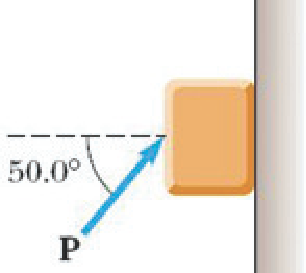
\includegraphics [scale=0.6]{./latex/eps/1_5_14_image_1-eps-converted-to.pdf}
\end{center}

Balok dengan massa 3.00 Kg ditekan ke atas pada dinding dengan gaya \textbf{P} yang membentuk sudut $50^{0}$ terhadap horizontal. Koefisien gesek statik antara balok dengan dinding sebesar 0.25. Tentukan nilai yang mungkin dari besar gaya \textbf{P} agar balok tetap stasioner.

